%
% instructions for "compiling":
%   latex main (first pass, also generates .aux file for bibtex)
%   bibtex main (generates .bbl file with bibliography)
%   latex main (second pass, incorporates bibliography)
%   latex main (do this if you still get messages about labels
%      having changed or missing references)
% to generate/view/print postscript:
%   dvips -o main.ps main 
%   gv main.ps (to view)
%   lpr main.ps (to print, or print from "gv")
% to generate/view/print PDF:
%   dvips -Pcmz -Ppdf -j0 -G0 -o main.ps main
%   ps2pdf main.ps main.pdf
%   acroread main.pdf (to view/print)
%   
\documentclass[11pt]{report}

% miscellaneous packages
% FIX THIS -- can add to or change, but these are useful
%
% uncomment the following if your input includes characters other than
% 7-bit ASCII (e.g., accented characters)
%\usepackage[utf8]{inputenc}
%
\usepackage{amsmath}
\usepackage{graphicx}
\usepackage{tikz}
\usepackage{moreverb}
\usepackage{url}
\usepackage{subcaption}
\usepackage{verbatim}
% double spacing
\usepackage{setspace}
\doublespacing

% hyphenation
\usepackage[english]{babel}
\selectlanguage{english}

% allow more figures on a page
\setcounter{topnumber}{10}
\setcounter{bottomnumber}{10}
\setcounter{totalnumber}{10}
\setcounter{dbltopnumber}{10}
\def\topfraction{1.0}
\def\bottomfraction{1.0}
\def\textfraction{0.0}
\def\dbltopfraction{1.0}

% margins
%\usepackage[letterpaper,top=2.0in,bottom=1.5in,left=1.5in,right=1.0in]
%	{geometry}
\usepackage[top=2.0in,bottom=1.5in,left=1.5in,right=1.0in]{geometry}

% set up to put page numbers in header
\usepackage{fancyhdr}
\pagestyle{fancy}
\lhead{}
\chead{}
\rhead{\rm\thepage}
\lfoot{}
\cfoot{}
\rfoot{}
\renewcommand{\headrulewidth}{0pt}
\renewcommand{\footrulewidth}{0pt}

% author, title, and date
% FIX THIS
\newcommand{\theAuthor}{Alexander Hansen}
% FIX THIS -- but be sure to leave in \par if title might exceed
%   one line -- otherwise space between lines will be wrong
\newcommand{\theTitle}{Modified Huffman Code for Lossless Compression and Bandwidth Optimization and Applying Genetic Algorithms to Generating Paintings Based on Images \par}
% FIX THIS
\newcommand{\theDate}{April 04, 2018}

\newlength{\WidthOfX}
% do not set here -- set just before use so we get the right font size
%\settowidth{\WidthOfX}{X} 
\newenvironment{TitlePageList}
{\begin{list}{}{%
  \setlength\leftmargin{0pt}%
  \setlength\labelwidth{10pt}%
  \setlength\itemindent{0pt}%
  \let \makelabel\descriptionlabel%
}}
{\end{list}}

% FIX THIS -- can put additional macro definitions here

%----------------------------------------------------------------------

\begin{document}
\tracingall


\pagenumbering{gobble}

%
% spacing could probably be improved
%

\begin{center}

\bigskip

\begin{Large}
\textbf{\theTitle}
\end{Large}

\bigskip

\begin{large}
\theAuthor
\end{large}

\bigskip
\bigskip

\textbf{Abstract}

\end{center}

\noindent
This thesis contains two projects. A modified Huffman code is presented as a lossless method to compress common traffic types. We posit the usage of compression benefits instead of just frequency of occurrence, as is common in Huffman codes, as the priority of each node when constructing the Huffman tree. We show the effectiveness of this method on common data transmission types and describe what would be needed for adoption of this new algorithm. 

We explore genetic algorithms as a method to create paintings based on images. We find a balance between computational work required and visually pleasing results to the algorithm, prioritizing aspects of the parameter space based on their impact on the painting and how they impact computational workload. 




\clearpage
%
% spacing could probably be improved
%
\begin{center}

\bigskip

\begin{Large}
\textbf{Acknowledgments}
\end{Large}

\bigskip

\end{center}

%FIX THIS --- thank your advisor, etc., here.
Thanks to Dr. Mark C. Lewis, my thesis advisor, and Dr. Paul Myers, my academic adviser, for being ever-present entities in my education at Trinity University.



\clearpage
\begin{singlespace}

\begin{center}

\textbf{\theTitle} 

\vspace*{\baselineskip}

\theAuthor 

\vspace*{\baselineskip}

A departmental senior thesis submitted to the \\
Department of Computer Science at Trinity University \\
in partial fulfillment of the requirements for graduation \\
with departmental honors. 

\vspace*{\baselineskip}

\theDate

\vfill

$\overline{\mbox{\rule{0in}{0.16in}Thesis Advisor~~~~~~~~~~~~~~~~~~~~~~~~~~}}$ 
\hfill
$\overline{\mbox{\rule{0in}{0.16in}Department Chair~~~~~~~~~~~~~~~~~~~~~~~~}}$ 

\vspace*{2\baselineskip}

$\overline{\mbox{\rule{0in}{0.16in}
~~~~~~~~Associate Vice President~~~~~~~~
}}$ \\
for \\
Academic Affairs

\end{center}

\vfill

\begin{small}

\settowidth{\WidthOfX}{X}

% FIX THIS comment/uncomment \item lines so correct box is checked
\noindent
Student Copyright Declaration: the author has selected the following
copyright provision:

\begin{TitlePageList}
%\item{[X]}
\item{[\hspace*{\WidthOfX}]}
This thesis is licensed under the
Creative Commons Attribution-NonCommercial-NoDerivs License, which
allows some noncommercial copying and distribution of the thesis,
given proper attribution.  To view a copy of this license, visit
\url{http://creativecommons.org/licenses/} or send a letter to Creative
Commons, 559 Nathan Abbott Way, Stanford, California 94305, USA.

%\item{[X]}
\item{[\hspace*{\WidthOfX}]}
This thesis is protected under the provisions of U.S. Code Title 17.
Any copying of this work other than ``fair use'' (17 USC 107)
is prohibited without the copyright holder's permission.

%\item{[X]}
\item{[\hspace*{\WidthOfX}]}
Other:

\end{TitlePageList}

\vspace*{2\baselineskip}

\noindent
% FIX THIS comment/uncomment \item lines so correct box is checked
Distribution options for digital thesis:

\begin{TitlePageList}

\item{[X]}
%\item{[\hspace*{\WidthOfX}]}
Open Access (full-text discoverable via search engines)

%\item{[X]}
\item{[\hspace*{\WidthOfX}]}
Restricted to campus viewing only (allow access only on the Trinity
University campus via \url{digitalcommons.trinity.edu})

\end{TitlePageList}

\end{small}

\end{singlespace}


\clearpage
%
% spacing could probably be improved
%

\begin{center}

\vfill

\begin{Huge}
\textbf{\theTitle}
\end{Huge}

\bigskip \bigskip \bigskip

\begin{huge}
\theAuthor
\end{huge}

\vfill

\end{center}


\tableofcontents
\listoftables
\listoffigures



\clearpage
\pagenumbering{arabic}

% TODO: Average increase based on iterations, based on strokes, based on..etc.
% Average time increase based on iter..stroke...etc%  the painting curves... Get control function: takes in the start and end pFixoints, generates two other points along the line that are within reason4

% make background white
% run tests in a sane manner with decent straight lines
% percent increase over
%figure out optimal minimum settings

\chapter{Modified Huffman Coding for Lossless Compression and Bandwidth Optimization}
\section{Introduction}
This project is a compression algorithm based on the Huffman code. We maximize the amount of tokens in the tree in exchange for a smaller compressed message. We avoid having to store the entire Huffman tree with the compressed message by storing it separately, giving an identification number to it and prepending all messages compressed using that code with that identification number, so it can be used to decode it later. Instead of constructing a Huffman code for every single file we compress, we construct a number of generalized Huffman codes based on a category of data and assign each an identification number. These codes and identification numbers together become a ``data context''. We implement a program that holds many data contexts and assigns the best one to each input message and observe how much we can compress messages and how quickly the messages can be decoded

\subsection{The Problem}
Cisco estimates that in 2016, over 96,000 petabytes of data were transferred across networks around the world.\cite{cisco} This is up from 72,000 petabytes in 2015 and for an even more extreme comparison, 12 petabytes in 1998. Clearly, internet traffic is increasing at a great pace. As internet traffic increases, consumers are sending more and more web requests from their client devices every day, with more and more devices to send from. This creates a challenge for those who maintain servers that handle these requests. Savings of kilobytes or even just bytes can add up to have a significant impact on total bandwidth usage when requests are being processed en masse. If there were a way to more effectively compress data before sending it to the client, provided it is quick at both compressing and decompressing and is relatively easy to implement, the savings in bandwidth could be huge, thus providing benefit to any implementing networks. We suggest a compression algorithm and implementation that meets these criteria. 

\subsection{Common Transmission Types}
The majority of traffic on the internet is either text, image, video, or audio. This paper will focus on a text implementation due to the ease of representing text on paper. However, it has already been shown that Huffman code techniques can be used to compress images, video, and audio as well.\cite{huffaudio}\cite{huffimage}\cite{huffvideo} The algorithm we present can therefore also be used on these formats.

Recently, the concept of minimizing Javascript of other web languages has become more and more important. If a large company with a website that is accessed a lot is able to minimize their payload, or filesize of their webpage, they could save lots of bandwidth. Our solution can be used to compress code very efficiently, so this is another reason for focusing on text in our implementation and examples.

What is important is that all common network traffic types can be tokenized, and when tokenized, there is at least some redundancy present. This is when minimum redundancy codes such as the Huffman code are most useful and effective. Note that there is a lot of redundancy in Javascript code (and most code) in the form of variable names, bracketing, keywords, etc., making it a great target for Huffman-based compression. Even if there is not that much redundancy, a Huffman code can be used to hold sets of equivalently occurring tokens to save memory.\cite{huffmemeffic} A Huffman code based solution is therefore very adaptable to the terrain of modern data transmission.

\subsection{Proposed Solution}
Bandwidth is clearly the core concern. We could minimize bandwidth with all sorts of lossy compression, but lossy compression is not acceptable in an algorithm designed for all kinds of web traffic and could result in corrupted data. We seek to minimize bandwidth usage with only lossless techniques.

As memory and data storage device prices decrease every year, it is becoming less and less important to be efficient in space complexity.\cite{mccallum} The traditional Huffman code is fairly conservative in its use of space. We seek to take advantage of this modern trend by inflating the size of the compression and decompression programs themselves in exchange for a smaller compressed file size and thus better compression ratio. Transmitting this smaller file will then use less bandwidth.

From a high level perspective, the version of the Huffman code we present has two major deviations from the original specification. The addition of a data context and the offloading of the Huffman code tree itself into the implementation specification, saving the output file from having to store the entire tree. The addition of a data context has been discussed before, but it has not been as large or offloaded as ours is.\cite{huffimage} We also introduce the concept of a compression benefit. That is, the benefit of compressing something big is more than compressing something small. This will be discussed more later.

A Huffman code is constructed by breaking apart an input message into tokens and constructing a tree based on those tokens and how frequently they occur, with the most frequently occurring tokens at the top of the tree. This tree can then be traversed to encode or decode messages. An example of a traversal represented as a binary string is shown in Figure \ref{fig:hufftraversal}. In this example, $0$ represents going to the left child and $1$ represents going to the right child. The tree itself and the traversal are then written to the disk in an efficient manner, providing a compressed file. If the tree grows too large, then writing it to the output file could make the output file larger than the original input. This is why the Huffman code's most common used method of tokenizing an input is by the letters and symbols used in English, ensuring that no more tokens than the English alphabet and some other symbols are encoded. As this sort of memory conservation is not important in our implementation, we want to choose a less granular token. In our example of English text, we could choose a word or small phrase. We will use a word, as implementing a decision algorithm for determining what constitutes a small phrase is not the focus of this paper, but such an algorithm could be a great addition.

With these less granular symbols, in our case words, we can then construct a much larger Huffman code tree based on the text. This tree should not be based on one individual file, rather, a corpus based on some genre of text. These subsets should be similar in genre, providing a more accurate tree. As an example, if one were to construct a Huffman code tree on all papers submitted to a computer science journal and then use that code to compress the next submitted paper, it would probably do a decent job. If that code was then used to compress all tweets made in the past hour, it would probably not compress that file very well, barring some extreme coincidence. This genre-generalized Huffman code tree is the ``data context'', or context of the data being transmitted.

We then take this very large data context, created from a corpus of computer science academic papers, and store it in the encoding/decoding program with an identification number. The identification number is a fixed-length message before the actual encoded message that specifies which data context was used to encode this message. The output file then does not have the large Huffman code tree in it taking up space, rather, it has an identifier for a data context that it will be paired up with when it is received and decoded.

There is also the consideration of benefits. If the word ``a'' occurs extremely frequently in the input, it will be in one of the top levels of the Huffman code and be compressed down to a very small size. However, if we compress the word ``the'' down to that same small size, even if ``the'' is less frequent, we are potentially (depending on the frequency of occurrence of ``the''), going to be compressing more efficiently. For the sake of example, assume a one-byte letter size and the token is on the third level of the tree, meaning a three-bit compressed token size. We would be removing 5 bits from the representation of the token ``a'' and 21 bits from the representation of the token ``the''. The benefit of compressing a symbol is the frequency at which it occurs times the size of that token. We then use these benefit values instead of the normal frequency value used by a standard Huffman code.

As decoding a compressed file using a Huffman code is very fast, this file can be decompressed quickly.\cite{fastdecode} We also considered using different branching factors to minimize the depth of the tree, but this turns out to have no real impact on output file size. %TODO citation here

\begin{figure}
\centering
    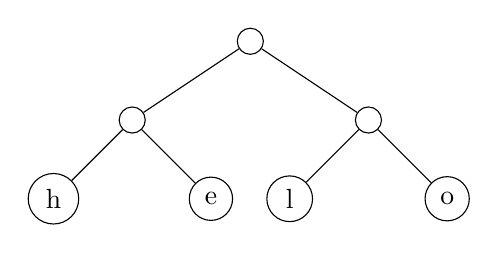
\begin{tikzpicture}
    \node [circle, draw] (e) at (1, 0) {};
    \node [circle, draw] (l) at (2.5, -1) {};
    \node [circle, draw] (h) at (-0.5, -1) {};
    \node [circle, draw] (o) at (-1.5, -2) {h};
    \node [circle, draw] (w) at (0.5, -2) {e};
    \node [circle, draw] (r) at (3.5, -2) {o};
    \node [circle, draw] (d) at (1.5, -2) {l};
    \draw  (e) edge (h);
    \draw  (h) edge (o);
    \draw  (h) edge (w);
    \draw  (e) edge (l);
    \draw  (l) edge (d);
    \draw  (l) edge (r);
    \end{tikzpicture}
    
    0001101011
    
    \caption[Huffman code example]{A rudimentary Huffman code tree with a corresponding binary string that encodes the string ``hello''. A ``0'' in the string corresponds to going to the left child of a node, and a ``1'' corresponds to going to the right. }
    \label{fig:hufftraversal}
\end{figure}


\section{Implementation and Methods}

\subsection{Specification}

The implementation of this algorithm has two parts: a client and a centralized server that keeps track of data contexts. The client needs to have access to a set of standard data contexts (Huffman code trees), their identifiers, and have the ability to traverse them to decode or construct a lookup table to encode a message. The server needs to store all data contexts and their identifiers and provide updates to the clients when needed.

The client as described here is not the typical web definition of a client as a browser, it is an implementation of our algorithm to encode or decode messages. The clients will requests new contexts from the server if they come across a context identifier for which they do not have the context. The client will also be tasked with determining which context, given its current inventory, is most efficient. The simple, and slowest, way to do this is to compress the message with every potential data context and pick the best one. There are much better ways to do this using genre classification, which is an entire field of its own. What is important here is that the process of deciding which context would be optimal does not have to be a brute force solution like what we are using. We used that in our implementation that for simplicity's sake, though. Because the decision of which data context to use must be done when encoding, the process of encoding will indeed be slower than decoding. This is okay, as it could be done in advance (not on the fly as requests are made) to all files being sent. For dynamically generated files, a smarter classification algorithm would be needed to assign an optimal data context on the fly.

%TODO: out of place?
An encoded file consists of the context identifier, the compressed data, and any tokens that were not found in the data context at the end. This is necessary because, as the contexts are not generated based on the input file itself, it is possible for an input file to have tokens in it that are not in the context. There will be a node in the data context that is in the least likely position, a leaf at the farthest level of the tree, that will be a placeholder. The tokens not present in the data context are then stored in their original form at the end of the file, in the same order that the placeholders occurred. This does mean that if a very malicious input message were to somehow circumvent all available contexts and contain a large amount of tokens that no context contained, it would be possible for the message to actually expand instead of being compressed. This is, however, both extremely unlikely and could be checked by comparing the output message size to the input message size and opting not to compress in this case.

The context identifier at the beginning of the file would be however long the implementers feel necessary for it to cover all contexts they would desire. This sort of decision has been historically difficult to make correctly, as the popularity of a particular system is hard to gauge at its inception (e.g. IPv4). In our implementation, it was three bytes, with an option to check the end of the file for more version info if all three bytes were 255. 

\subsection{Advantages}
The solution to the problem of bandwidth optimization is the primary advantage. This algorithm can cut down on file sizes in transmission by immense amounts. This algorithm also can be implemented easily, without much more difficulty than a regular Huffman code. This is important, as the adoption of this algorithm would require browsers to implement decoders and servers to implement encoders (clients and servers here referring to the web sense of the words, not our specification's definition). It is also adaptable to many different data formats and allows for a lot of data contexts, so a data context can fit a specific input message very well.

\subsection{Disadvantages}
Corner cases do exist. It is hypothetically possible for a file to expand, or get abysmal compression. We do avoid this as much as possible, but there will theoretically always be some heinously complicated input that could not be compressed very efficiently. This would not happen in general, though.

The disk space required to store so many data contexts could become very large, especially when accounting for different data types (audio, video, etc.). We assume disk space is not an issue, however, and disregard this.

Lastly, this algorithm is not very good at handling random data or noise. If a person is browsing their computer late at night and drifts off to sleep, their head could hit the keyboard and generate the string ``ugibigbnhdfvbsmdofu''. This would most likely not belong to many contexts, and if it did, that context would not fit the rest of the text very well. This is not too big of a problem, though, as it will just remain uncompressed via the placeholder nodes in the context. The implementer also has the choice to be more smart about these situations and perhaps resort to a different compression algorithm.

\subsection{Our Implementation and Strategy}

Our implementation used the programming language Rust, for its speed and ease of implementing low-level data structures safely (i.e. without memory leaks or things of that nature).

The construction of this tree can be seen in the appendix as Figure \ref{fig:newdatacontext}. First, the corpus is split up on spaces. In a more efficient implementation, punctuation would also be its own token, but I have omitted this from the appendix for brevity. These tokens are then stored as tuples with their benefits, calculated as their length times their size. These tuples are then inserted into a priority queue/min heap strucure which is popped repeatedly to constructed the Huffman code. A lookup table for quicker encoding is constructed from the code for all tokens it contains. Finally, some identifier (arbitrary at this point) is attached to the code to form a data context. 

For encoding, each token is found in the lookup table with its corresponding encoded form. For decoding, the data context traverses the Huffman tree following the traversal prescribed by the binary encoded file. This means that encoding is $O(n)$ where $n$ is the number of tokens in the input and decoding is $O(m)$ where $m$ is the size in bits of the encoded message. Both are very fast operations.

\section{Results}
We constructed a few data contexts that are representative of data frequently transmitted over the internet, namely minified Javascript, English text sourced from novels, and social media English text (a corpus of tweets). We compressed another sampling of texts from the same genre as the data context and averaged the compression ratios to get the values seen in Table \ref{table:compressionResults}.



One particular advantage of using a Huffman coding in this manner is the bit-level output of the algorithm. As the actual implementation of characters varies by application (some applications will have single-byte char sizes, some have two-byte char sizes, systems that support Unicode have four-byte char sizes). The compressed size will always be the same number of bits, but the ratio can depend on how big a character or token is in the original file. The encoding and decoding part of this program took under one-fiftieth of a second total on my (somewhat slow machine, even with extremely large data contexts (for example, the English Novels context contained over $50,000$ tokens). 

Great compression results can be had with this compression algorithm, especially in the realm of highly redundant data like code (e.g. Javascript). It would just need to be adopted by both servers and clients for it to be practical. 

\begin{table}[h]
\centering
\caption[Compression Results]{Some compression results using data contexts. The ratios are the compressed size over the original size, both in bits. In the ``Benefits Ratio'' column is the result for the calculation using benefits, and in the ``No Benefits Ratio'' column, a standard Huffman code using just the frequency of token occurrence was used.}
\label{table:compressionResults}
\begin{tabular}{lll}
                     & Benefits Ratio & No Benefits Ratio \\
English Novels       & 0.29214        & 0.41200           \\
English Social Media & 0.38830        & 0.42221           \\
Javascript           & 0.23819        & 0.38194          
\end{tabular}
\end{table}

\section{Future Work}
We hope to construct many more data contexts for varying data types and investigate exactly how many contexts would be needed to adequately cover all common data transmission types. We also hope to implement the encoding and decoding programs as browser and server plugins, enabling transmission of data compressed in this manner and supporting adoption of this algorithm.




% problem

%TODO: it would be fun to create an image based on one photo and do the fitness with respect to another photo

%TODO: appendix of photos run through the painter
%TODO: Insert a narrative of finding the balance of computational work and good fitness/visual results

\chapter{Applying Genetic Algorithms to Generating Paintings Based on Images}
\section{Introduction}

This project explores the application of genetic algorithms to generating paintings based on photos. We find various combinations of parameters for our genetic algorithm that strike a balance between computational work and visually pleasing and accurate results. 

\subsection{Background Information}
The subject of generating paintings based on algorithmic operations applied to computers has been studied before in great depth.\cite{synergistic}\cite{monet}\cite{organicpainting} These approaches are highly effective and expressive, but some can be stylistically limited due to their deterministic nature of analysis. In the case of both \cite{synergistic} and \cite{monet}, they analyze features from the original image, such as color or edge location, and abstract them into something that can become a stroke or collection of strokes and represent them in a table. The painting algorithm draws from this table to ensure the feature is represented in the final rendered painting. This is the approach of most painting algorithms that are based on an original image. Those other algorithms which paint images based on no original reference image, such as \cite{organicpainting}, are a different problem than this project, so they will be referred to sparingly. 

As it is hard to say in art whether one approach is better or worse, this project seeks not necessarily to improve upon the previous work but to provide another entirely different tool for generating paintings based on a reference image. We utilize machine learning, specifically a genetic algorithm, to create a large amount of paintings and then evolve them into one, particularly accurate, painting. This accuracy is determined by a fitness function which is discussed later. 

The concept of a genetic algorithm was originally proposed by A.S. Fraser with the intent of being able to computerize and simulate evolution.\cite{fraser1957simulation} Originally, it was much more focused on the mutation and mating aspects of it, and less on the fitness definition and iteration. In applying genetic algorithms to art, however, a creative use of a fitness function and a mutation function are required. 

Much work has been done on genetic algorithms, and they seem to contain an inherent quality that makes them good at optimization problems. This can be seen in the amount of publications across many diverse fields using genetic algorithms to optimize their problems. Some examples are molecular geometry calculations,\cite{molecular} electromagnetic design tools,\cite{electro} course scheduling.\cite{courses} There is much more work out there exemplifying this optimization characteristic. \cite{genetic1}\cite{genetic2}\cite{genetic3}\cite{genetic4}\cite{genetic5}

Genetic algorithms are often applied to optimization problems in this way because they are able to find optimal solutions without necessarily knowing why they are optimal. In problems where there are features that can be evaluated and weighted based on how good or bad they are with respect to the final product, genetic algorithms are able to find optimal arrangements of these features. We apply this to paintings, as every stroke can be viewed as a feature and evaluated in this way. Some work has been done on applying genetic algorithms to art and in very interesting ways. Karl Sims has published a paper and created an art exhibit using one.\cite{sims} He, too, struggles with large parameter spaces in his work and discusses some ways around them, but his process is not based on a reference image as ours is, so we cannot take advantage of these approaches. %TODO study these

Sims also has an exhibit where there are sixteen different paintings, and visitors to the exhibit can select the most visually appealing ones. Their features are then mixed to create the next generation of paintings. This is a good demonstration of the idea behind genetic algorithms.

Other work on using genetic algorithms with art include Roger Johansson's implementation in Javascript of a genetic algorithm to approximate the best arrangement of fifty polygons to replicate the Mona Lisa with great success.\cite{monalisa} This project can be viewed online. \footnote{It can be viewed here: https://chriscummins.cc/s/genetics/}


\section{Implementation}

\subsection{Applying a Genetic Algorithm to Painting}
There are three core parts to this project: the generation function, the genetic algorithm, and the rendering. Paintings are a struct represented by a collection of strokes, which is a struct with a start point, an end point, a width, and a color. 

The genetic algorithm itself has five parts: the selector function, which selects which of the population to mate; the fitness function, which defines the fitness of a painting; the crossover function, which defines how two paintings interact to create a child; the mutation function, which randomly mutates a painting; and the simulator, which iterates the genetic algorithm according to some given properties and kills off stochastically.

The structure of the program, from a high level, is as follows:
\begin{enumerate}
    \item The generator function generates $n$ initial random paintings.
    \item The selector function selects $m$ of the initial random paintings to mate and produce child paintings.
    \item The crossover function takes two selected paintings and combines their strokes, half from one and half from the other, to create a child painting. It repeats this process until all of the selected paintings have been mated.
    \item Another selector function selects $o$ random members of the population.
    \item The mutation function mutates these $o$ members.
    \item The simulator then stochastically kills off $m$ paintings from the population.
    \item Go back to step 2 and repeat until a predetermined number of iterations has been met.
    \item Render the most fit, according to the fitness function, of the population and output it as the final result.
\end{enumerate}

\subsection{The Fitness Function}
This paper will frequently refer to the ``fitness'' of a painting. This is a value determined by the fitness function. It is therefore crucial to explain first, as the rest of the discourse in this paper relies on this concept. The fitness function gives us an integer value for how ``good'' a painting is with respect to the original photo. This allows the various parts of the simulator to address photos by how fit they are and make decisions accordingly. It also provides us with a quantitative metric with which to compare the effectiveness of various approaches and tweaks to our program.

In our problem, we want to take an image and turn it into a painting. One of the most basic concepts of how accurate a painting is to a given reference photo is how far off the color is of every pixel. For example, given the RGB values of original photo pixel located at $(1, 1)$ as $(255, 254, 255)$ and the corresponding painting pixel located at $(1, 1)$ as $(255, 255, 255)$, we can see that the $G$ value is one pixel off from the original. This gives it an ``unfitness'' of $1$. We can take the inverse of this to get the fitness. The inverse is the maximum possible difference ($255 + 255 + 255 = 765$) minus the actual difference ($1$), so $765 - 1$. Therefore, this particular pixel in the painting has a fitness of $764$. The fitness value of a painting is the sum of the fitness of every rendered pixel in comparison to the original photo.

Note that the fitness function does not rely on mutating any data, only referencing the two images. This means that it is easily implemented in parallel, a feature that is important in executing genetic algorithms in a timely manner. The actual code for this function can be seen in the appendix as Figure \ref{fitnesscode}. 



\subsection{The Rendering Function}

Rendering a painting is as minimalist and intuitive. From the start point to the end point of every stroke, a line is drawn with the stroke's color. This line has the width of the stroke's width. There is no actual paint simulation or anything particularly advanced happening here. This is because the discoloration of paint or lighting could interfere with the fitness function's ability to accurately compare the color of a stroke to the original photo. 

The rendering function is important to this project because it is used in the calculation of the fitness and therefore the assessment of the genetic algorithm's progress and quantitative results.


Figure \ref{fig:refvsfinal} shows an example of a rendered painting with it's original image next to it. 
\begin{figure}
\begin{subfigure}[t]{.5\linewidth}
      \centering
      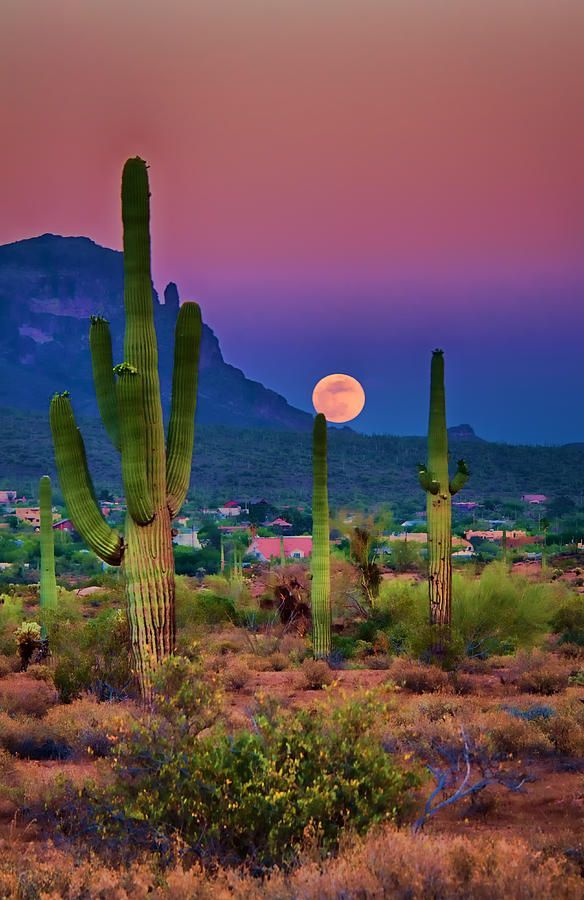
\includegraphics[width=0.4\linewidth]{reference.jpg}
  \end{subfigure}%
  \begin{subfigure}[t]{.5\linewidth}
      \centering
      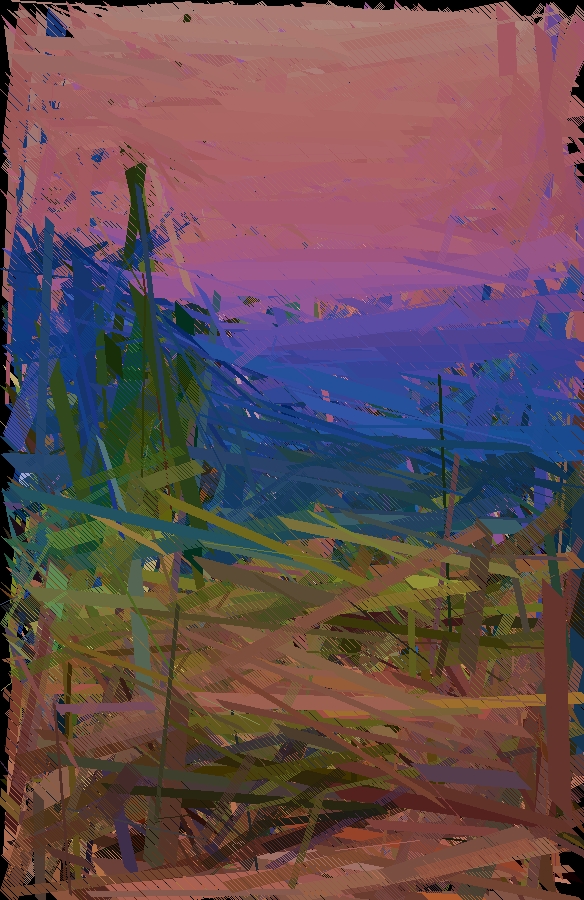
\includegraphics[width=0.4\linewidth]{informed.png}
  \end{subfigure}
  \caption{A rendered painting with its original reference image to the left of it}
    \label{fig:refvsfinal}
\end{figure}


\subsection{The Generator Function}
The generator function is the function that generates random paintings for the initial population of the genetic algorithm. Originally, it was truly random, generating completely random strokes with completely random parameters and combining them into a painting. This was not good enough. The parameter space of the problem is too large. Strokes have color, length, position, width, etc., and starting with truly random strokes puts us so far away from an optimal solution that it takes the genetic algorithm far too many iterations to get a desirable result. We instead created an ``informed'' random generator. In this improved generator, most aspects are still kept random but certain things are set to be more accurate by taking some features from the reference image. We limited the minimum and maximum length of strokes to be set by an argument passed in by the user, which minimizes the parameter space greatly. We also set the color of every stroke to be the color of the original image at its start position, and thus further shrank the parameter space. This proved to greatly increase starting fitness. Note that the fitness increase did not sacrifice the effectiveness of the genetic algorithm. The final fitness is a function of the starting fitness, as seen below. In Figure \ref{fig:informedvsrandom}, we introduce the ``fitness graph'' which is a graph of the maximum fitness at every iteration through an execution of our genetic algorithm, to show the difference in both fitness and final image when an informed random generation function is used versus a purely random one. 


\begin{figure}
\centering
  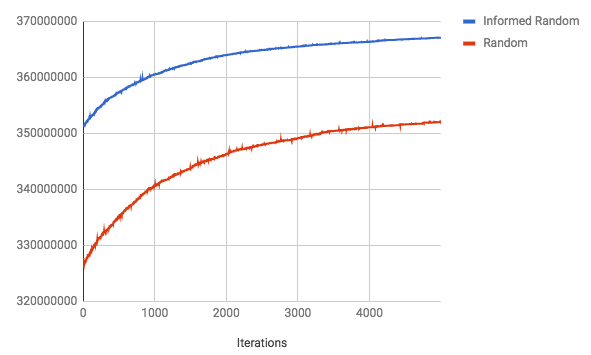
\includegraphics[width=\linewidth]{InformedvsRandom.png}
  \centering
  \begin{subfigure}[t]{.5\linewidth}
      \centering
      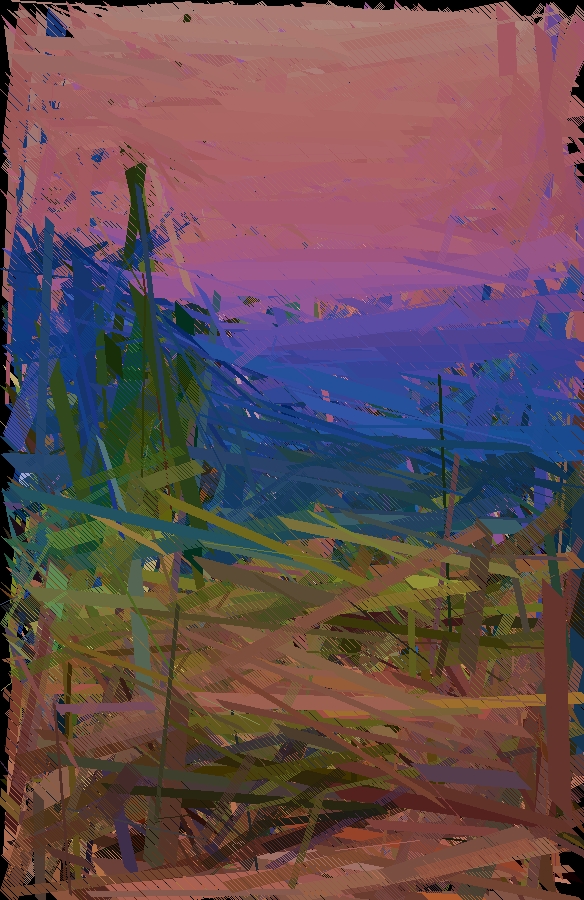
\includegraphics[width=0.4\linewidth]{informed.png}
      \caption{Informed random final result.}
  \end{subfigure}%
  \begin{subfigure}[t]{.5\linewidth}
      \centering
      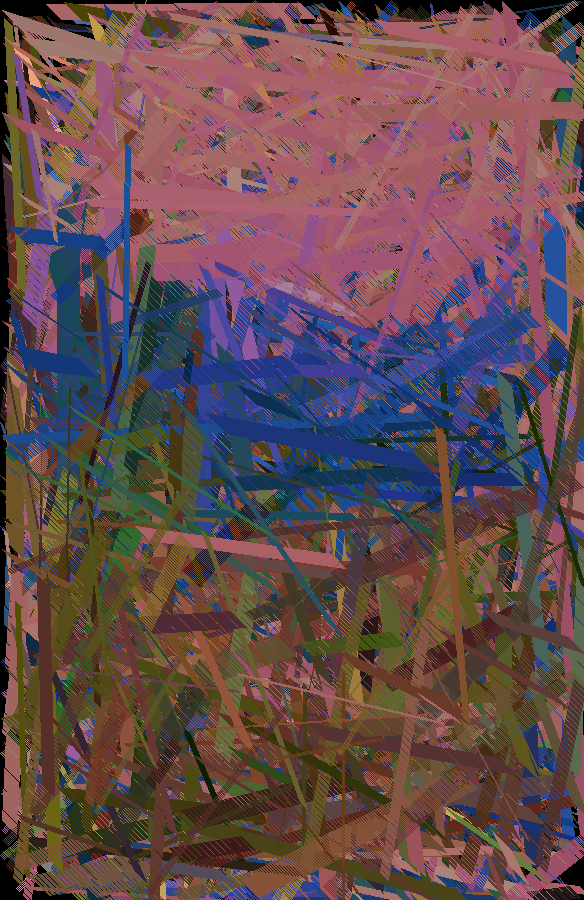
\includegraphics[width=0.4\linewidth]{random.png}
      \caption{Random final result.}
  \end{subfigure}
    \caption[Informed random generation compared with fully random generation]{The maximum fitness of every iteration's population using the informed random generation approach versus the non-informed approach, and their respective final results from the genetic algorithm after 5000 iterations.}
  \label{fig:informedvsrandom}
\end{figure}


\subsection{The Selector Function}
The selector function's job is to select which parents will mate to produce the children for the next iteration.

There are different kinds of selectors that are used in genetic algorithms. There is stochastic, which is random and is effectively useless for this application; there is tournament selection, which chooses $x$ members of the population at a time to participate in a tournament and picks the top $2$ most fit participants from that tournament (multiple tournaments can be run per iteration); fitness maximal selection, which selects the absolute most fit members to mate; and some other more obscure types.


The amount parents being selected to "mate" each iteration is an input to these selector functions. So, the maximize selector picks the top $x$ to mate, producing $\frac{x}{2}$ children. This is a parameter that we fixed to $\frac{n}{3}$, where $n$ is the total population size, producing $\frac{n}{6}$ of the population size children every iteration, and killing off $\frac{n}{6}$ as well. We tested a few other values, but ultimately fixed it to $\frac{n}{3}$ as it seemed optimal. This is discussed more in the results section. Fixing this value, although semi-arbitrary, provided consistency as we tested the other elements of the genetic algorithm's parameter space, which was already far too large. The maximize selector was our primary choice as it picks the most fit paintings and then uses them to create children. This can cause a phenomenon of a local maxima, but it still resulted in the highest fitness. That is, the local maxima level is higher in the maximize function than the highest fitness able to be achieved by other selectors in the same amount of time. This will be discussed more in the results section.

The tournament selector was the other selector we experimented with. It takes two parameters: the number of tournaments and the number of participants in the tournament. We fixed these values, again somewhat arbitrarily, to $\frac{n}{6}$ tournaments of size $\frac{n}{10}$. For a population size of $1000$, this would be $166$ tournaments of size $10$. This results in $1660$ fitness calculations per iteration, which is more than the maximize selector, but is often more efficient as it will select the same population member multiple times and access the cached fitness value. The scaling of the tournament selector is independent of the fitness increase, meaning it is not just a slower maximize selector.\cite{selectors} This means it could be resistant to the local maxima that the maximize selector can sometimes experience.


\subsection{The Crossover Function}
After a subset of the population has been selected to become ``parents'', they are passed into a crossover function. In the original definition of a genetic algorithm, this was a function that took the two parents' binary string representations and split them, combining part from one parent and part from the other.\cite{fraser1957simulation}

We approximate this process; instead of using a binary representation, we take half of the strokes from one painting and half of the strokes from the other, combining them. To maximize the increase in fitness, we compare the two potential combinations (parent one's first half, and then parent two's, or vice versa), and pick the best combination. This worked, but also made us more susceptible to local maxima, also known as Hamming walls. This will be discussed later in the results section. Because of this, this feature was removed. Some other versions of the crossover function exist, such as not taking exactly half from each painting and instead taking a random percentage from each that totals one hundred percent, but no major improvement in performance was shown using this method.
This new set of child paintings are then added into the total population.

\subsection{The Mutation Function}
After the child paintings are added to the population, a stochastic selector function selects a predetermined amount of paintings to mutate. We decided that we would pick a random parameter of a stroke and modify it by a predetermined ``mutation strength''. The code of our original implementation of the mutation function is available as Figure \ref{fig:origmutation} in the appendix. You will notice that in the end, this function, like the original crossover function, also makes a comparison to ensure a better fitness. The painting compares itself to its pre-mutated state and picks the more fit painting to return. This also made us more susceptible to Hamming walls, and was removed. The mutation strength is better as a relatively large value to help avoid Hamming walls. 

After the mutation occurs, a number of paintings equivalent to the amount of child paintings that were just added are stochastically selected to be ``killed'', or removed from the population.

\section{Results}
\subsection{Maximizing Fitness}
 Some of the most fit images generated based on the original reference image are below:
\begin{center}
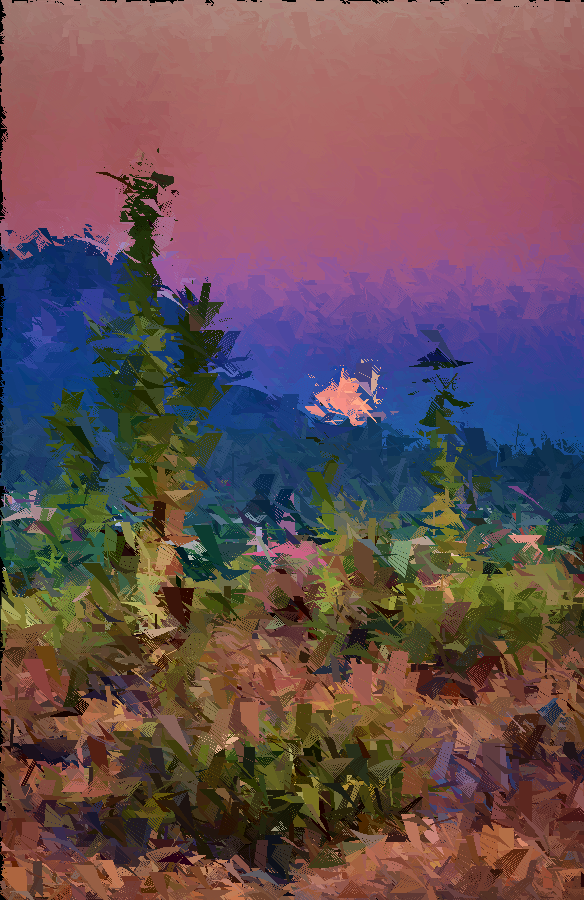
\includegraphics[width=0.4\linewidth]{final.png}
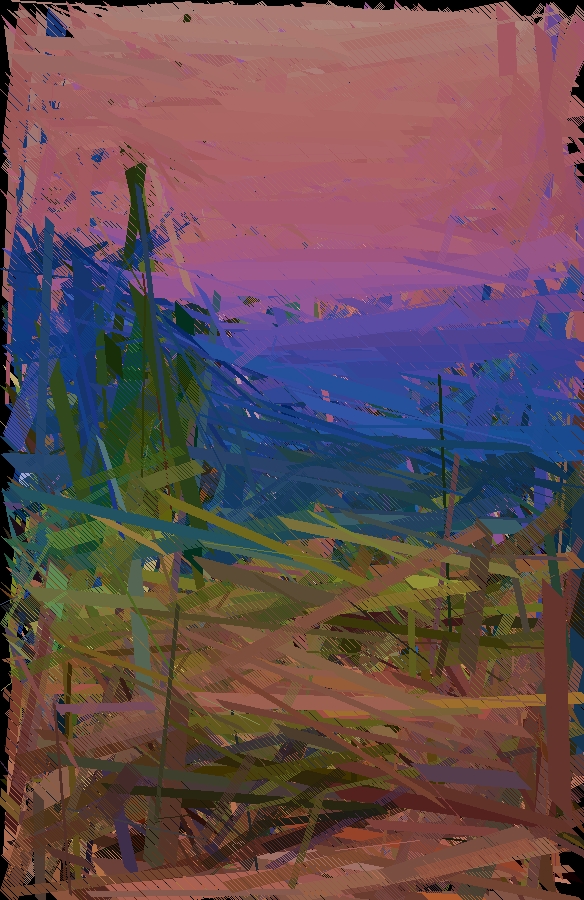
\includegraphics[width=0.4\linewidth]{informed.png}
\end{center}

More paintings can be seen in the appendix as Figure \ref{paintings}.

\subsubsection{Stroke Properties}
These two paintings ran for the same number of iterations. They show the increase in ``difficulty'' of arranging longer strokes versus shorter strokes. Through many tests, it has become apparent that a feature in a painting only shows up if the stroke length is less than that feature itself. The longer strokes tend to obscure the smaller details, like the moon in the background and some shrubbery in the foreground. In a much shorter time, a shorter-stroke painting is able to achieve a much higher fitness than another painting of longer strokes. So, one way to maximize fitness is to just have shorter strokes. Thinner strokes also have this effect but it is not as dramatically as shorter strokes. This ``impressionist'' style of painting strikes a great balance of computational work to good results, requiring much less computation for much more fit results.  For the sake of exploring other styles, we then chose to move on to the more challenging longer-stroke version and see how much improvement can be made.

\subsubsection{Selectors}
When trying to maximize fitness, it is intuitive to use the maximize selector. This is the selector that selects the most fit members of the population to mate for the next generation. It does increase the run-time dramatically, as at every iteration it must find the most fit members to mate, but the increase in fitness makes this trade-off worth it. Using the maximize selector to run a genetic algorithm for some amount of time hours will result in a higher fitness than using a tournament selector for the same amount of time. Technically, the tournament selector can get through many more iterations in the same time, but each individual iteration has a lesser positive impact on the fitness. 




\subsection{Hamming Walls}
\begin{figure}[t]
\centering
    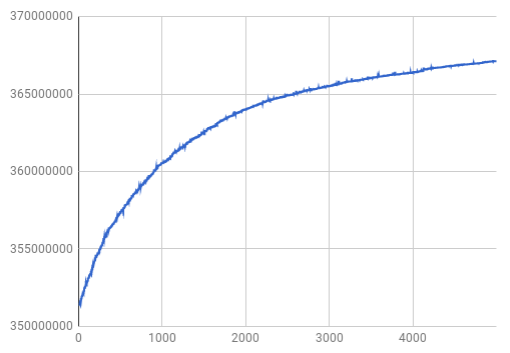
\includegraphics[width=0.6\linewidth]{2018-04-03-203542_510x353_scrot.png}
    \caption[Maximize selector fitness graph]{A graph of the maximal fitness throughout one execution of the genetic algorithm.}
    \label{fig:fitnessgraph}
\end{figure}
When looking at the fitness graph of an execution of our genetic algorithm, it takes a logarithm, or inverse-exponential, shape. This can be seen in Figure \ref{fig:fitnessgraph}. We postulate that this is due to a local maxima, or Hamming wall as they are called in genetic algorithms. This postulated maxima can be seen in Figure \ref{fig:hamming}. This is a place where an increase in fitness would require many changes to happen simultaneously.\cite{hamming} It could also be due to approaching the most optimal arrangement of strokes, but as a perfect fitness value is much higher than those values these lines are asymptotically approaching, this seems unlikely. 

More evidence for the existence of a Hamming wall can be seen in Figure \ref{fig:informedandrandom}. If the posited hamming wall was actually an optimal arrangement of strokes, then the fitness graph for the random generator execution should approach the same optimal arrangement as the informed random generator execution, around $368,000,000$, and then start to flatten out. Instead, it reaches its own Hamming wall around $351,000,000$. 
%Further evidence of hamming walls appears in the random graph - the initial slope is higher than the final slope of the random

\begin{figure}[b]
    \centering
    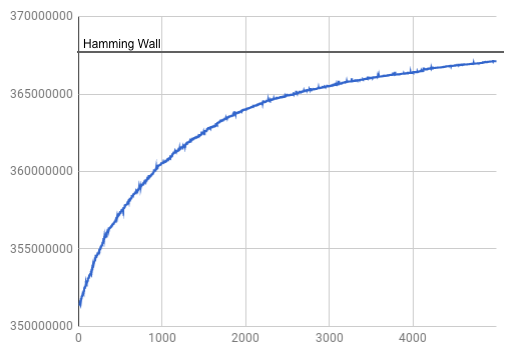
\includegraphics[width=0.6\linewidth]{hamming_graph.png}
    \caption[Visualized Hamming wall]{A fitness graph with a Hamming wall visualized. The Hamming wall is around fitness = $368,000,000$.}
    \label{fig:hamming}
\end{figure}

\begin{figure}
    \centering
    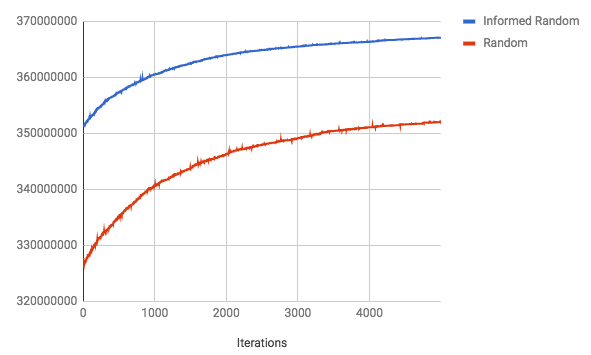
\includegraphics[width=0.6\linewidth]{InformedvsRandom.png}
    \caption[Informed random and random generator fitness graphs]{The fitness graph of two executions using an informed random and a random generator function.}
    \label{fig:informedandrandom}
\end{figure}
If one is familiar with Hamming walls, they may have heard of Gray coding. Hamming walls can be combated with something called Gray coding\cite{hamming} when using binary strings to represent members of the population. As our approach to using genetic algorithms on paintings does not use a binary-based representation, these methods of Gray coding are unfortunately not applicable. There may be ways to apply the strategies of Gray coding to our application, but they are not obvious at this point. 

Hamming walls, or local maxima in general, occur when an algorithm cannot see far enough in the future to make a change that will temporarily distance itself from its goal but eventually get it closer. When thinking about them in this sense, any part of our algorithm that greedily grabs the best option could be causing this phenomenon. The most obvious candidate is the maximize selector, which always grabs the most fit members of the population. For many iterations, that most fit member may not actually change at all, resulting in a lot of children with the same or extremely similar characteristics being added over and over again. Over a longer time, it is theoretically possible that a sudden mutation and more fit child could cause a spike and an overcoming of a Hamming wall.

Increasing the previously mentioned mutation strength would increase the probability of being able to overcome a Hamming wall. We tested raising the mutation strength until it was detrimental to the overall fitness and it never was able to overcome Hamming walls. %TODO graph

\subsubsection{Overcoming Hamming Walls with Selector Choice}

Discouraged by this Hamming wall, we turned to the tournament selector. It was touched on before, but for the sake of detail: the tournament selector works by selecting tournaments out of the total population. These tournaments each have $x$ participants, where $x$ is less than half of the population. It then picks the most fit two participants to make a child for the next iteration. This selector can sometimes be quicker than the maximize selector as you will only need to calculate the fitness of the tournament participants, not the entire genetic algorithm. This can also help avoid Hamming walls, as it will often not select the most fit or most optimal path for the next iteration. This results in a more flat, but perhaps more consistent, slope. 

Figure \ref{fig:tournament} shows the maximal fitness of every iteration using the tournament selector. Notice that it is more linear shaped, and less logarithmic, which is good when hoping to avoid asymptotically approaching a Hamming wall.
\begin{figure}
    \centering
    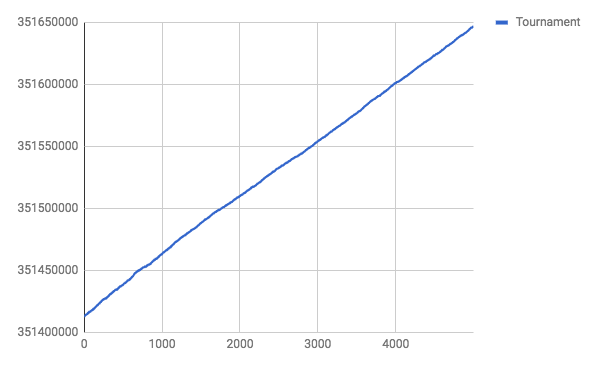
\includegraphics[width=0.6\linewidth]{Tournament.png}
    \caption[Tournament selection maximum fitness graph]{The maximum fitness of every iteration using the tournament selector. }
    \label{fig:tournament}
\end{figure}

This optimistically linear slope is immediately overshadowed when the tournament selector graph is plotted along with the maximize selector graph. This can be seen in Figure \ref{fig:tournamentvsmaximize}.
\begin{figure}
    \centering
    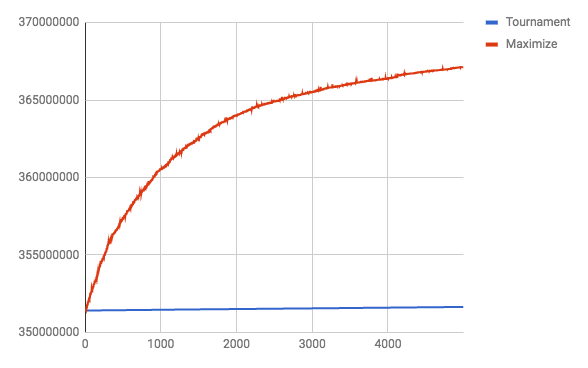
\includegraphics[width=0.65\linewidth]{TournamentvsMaximize.png}
    \caption[Tournament selector fitness graph versus maximal selector fitness graph]{The tournament selector's maximal fitness at every iteration graphed with the maximize selector's.}
    \label{fig:tournamentvsmaximize}
\end{figure}
Clearly, the maximize selector is far more effective. The postulated Hamming wall is so far above anything the tournament selector achieved in the same number of iterations. The genetic algorithm with a tournament selector would have to run for approximately $190,503$ iterations in order to overcome the one using a maximize selector's fitness. As the maximize selector took about $17$ hours to run $5000$ iterations and the tournament selector took about $13$ hours to do $5000$ iterations. The tournament selector would have to run for roughly $494$ hours, or $41$ days straight on our systems to even approach the Hamming wall of the maximize selector, assuming the linear slope would continue and it would not encounter its own Hamming wall at an earlier point. In that same time, the maximize selector would still be either slowly approaching the Hamming wall, or could be even higher than it. The amount of time required to achieve a comparable result with the tournament selector makes this approach not worth it unless running the genetic algorithm for a very long time. Lowering the tournament selector's parameters to do less tournaments or less participants in the tournaments does make it run faster but has a dramatically negative impact on the its slope. The increase in speed is not big enough to compensate for this negative impact on the slope. This can be seen in Figure \ref{fig:smallTourn}. The parameters of these two executions can be seen in Table \ref{table:tournTable}. 

\begin{figure}
    \centering
    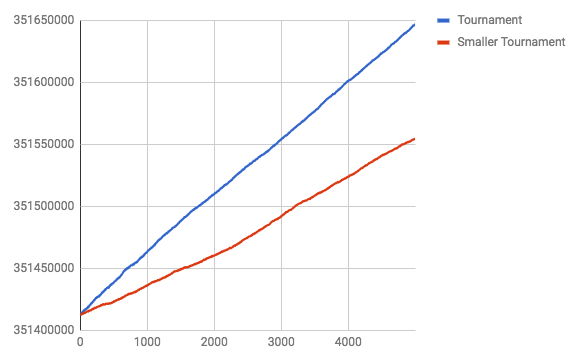
\includegraphics[width=0.6\linewidth]{SmallTournament.png}
    \caption[Tournament selector comparison]{The fitness graphs of our tournament size and a smaller tournament size.}
    \label{fig:smallTourn}
\end{figure}

\begin{table}[]
\centering
\caption{Parameters of the tournament selector executions}
\label{table:tournTable}
\begin{tabular}{lllll}
                   & Number of Tournaments & Tournament Size & Runtime  & Final Fitness \\
Tournament         & $\frac{n}{6}$         & $\frac{n}{10}$      & 13:12:52      & 351646879     \\
Smaller Tournament & $\frac{n}{10}$        & $\frac{n}{12}$      & 11:47:50      & 351554728    
\end{tabular}
\end{table}

From this test and similar ones, we deduced that it is not worth it to pursue smaller tournament parameters for more quick execution. The better balance of computational work and fitness is therefore in the larger tournament selector, but the best balance is still found in the maximize selector.

Due to these above factors, we moved on from tournament selection and used maximize selection for all tests after that.

\subsection{The Impact of Population Size}
\begin{figure}
    \centering
    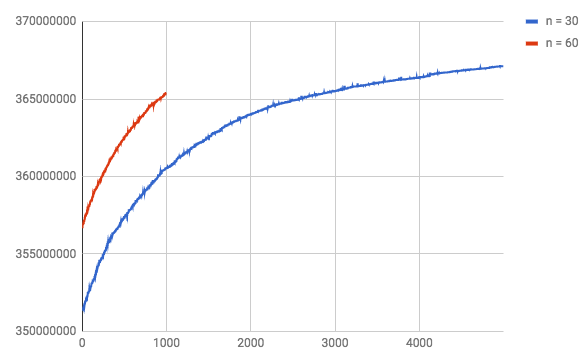
\includegraphics[width=0.7\linewidth]{popsize.png}
    \caption[Fitness graph of different population levels]{The fitness graph of two executions of the genetic algorithm: one with the population set to $n = 30$ and one with the population set to $n = 60$.}
    \label{fig:popsize}
\end{figure}
The size of the population in each iteration turns out to have a significant impact on the shape of the fitness graph. Unfortunately, it also increases the time it takes to execute one iteration greatly. 

For all executions mentioned up until this point, the population value has been set to $n = 30$. Figure \ref{fig:popsize} shows what happens when we increased the population size to $n = 60$, using our maximize selector. Unfortunately, it took so long to run, we were only able to run it out to a thousand iterations. But clearly the impact is massive. The slope at every point is higher and the initial fitness is higher. This makes sense from a conceptual perspective, with more population being generated in the beginning, there are more combinations of strokes and therefore a higher likelihood of more fit paintings being generated. Unfortunately, to run these $1000$ iterations took $69.18$ hours. Recall that running $5000$ iterations with $n = 30$ took only around $17$ hours. We found that doubling the population size  increases the amount of time required to run one iteration by a factor of $20.347$, on average. This means that increasing the population size is not as efficient as running a lower population for a longer time.

Some more examples of paintings and their reference images can be seen in the appendix as Figures \ref{fig:dadpics}, \ref{fig:guitarpics}, \ref{fig:hotairpics},  and \ref{fig:houstonpics}.


\subsection{The Impact of Iterations}
\begin{figure}
    \centering
    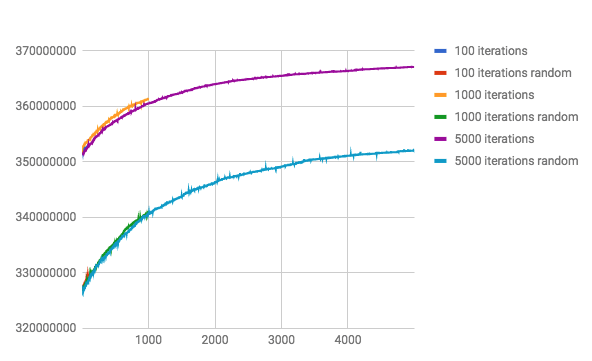
\includegraphics[width=0.8\linewidth]{randomIter.png}
    \caption[Fitness graph of multiple executions with varying amounts of iterations]{The fitness graphs of six executions, three of which used a random generator function and three didn't, of varying lengths (amounts of iterations).}
    \label{fig:iterationtests}
\end{figure}

The amount of iterations an execution has exerts a very predictable effect on the fitness graph. Shown in Figure \ref{fig:iterationtests}, the number of iterations merely determines how far along this logarithmic curve it goes. Note that even when a random generator is used, giving a lower fitness to start with, the pattern persists. 



\section{Future Work}
In the future, we hope to look into how to implement Gray coding for a project like this to avoid Hamming walls. New methods of combating Hamming walls may be needed in order to solve the problem in this context. We also hope to test more parameter configurations for our selectors, finding more optimal configurations. Lastly, we feel that implementing a more intelligent fitness function, maybe something that uses edge detection or something along those lines, could result in a more accurate evolution.
% Implementing Gray Coding
% Optimizing the selector/using tournament 
% More rigorous fitness function

\bibliography{refs}
\bibliographystyle{plain}

\appendix
% FIX THIS
%
% FIX THIS -- remove/change, just an example of a simple way to
%   include a lot of code (hello.c here)  
%

\chapter{Code Appendix}


\begin{figure}
    \caption{The original mutation function.}
    \begin{singlespacing} 
    \begin{small}
    \verbatiminput{mutation.rs}
    \end{small}
    \end{singlespacing}
    \label{fig:origmutation}
\end{figure}



\begin{figure}
    \caption{The function for creating a data context.}
    \begin{singlespacing} 
    \begin{small}
    \verbatiminput{newDataContext.rs}
    \end{small}
    \end{singlespacing}
    \label{fig:newdatacontext}
\end{figure}

\begin{figure}
    \caption{The function for calculating the fitness of a painting. Here, ``self'' is a painting.}
    \begin{singlespacing} 
    \begin{small}
    \verbatiminput{fitness.rs}
    \end{small}
    \end{singlespacing}
    \label{fig:fitnesscode}
\end{figure}

\begin{figure}
    \centering
    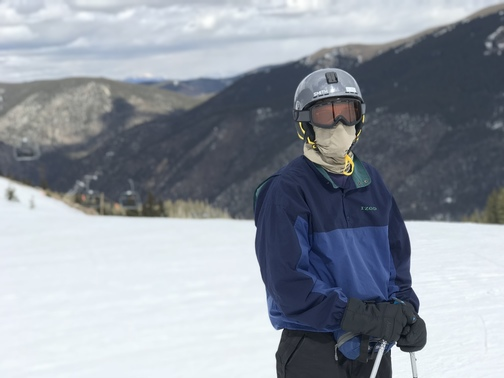
\includegraphics[width = 0.6\linewidth]{dad_pic.jpg}
    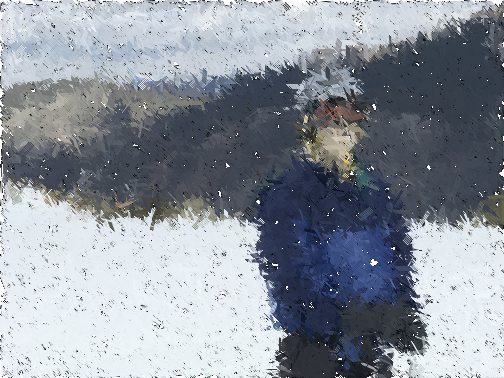
\includegraphics[width=0.6\linewidth]{dad_pic.png}
    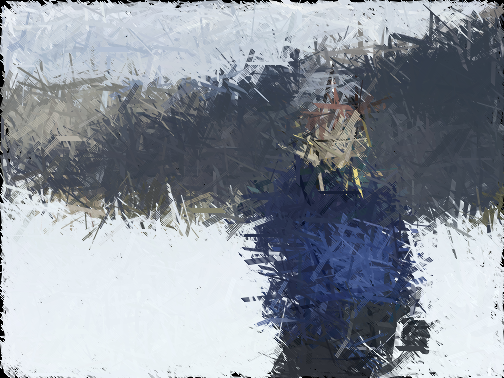
\includegraphics[width=0.6\linewidth]{dad_good_strokes.png}
    \label{fig:dadpics}
\end{figure}
\begin{figure}
    \centering
    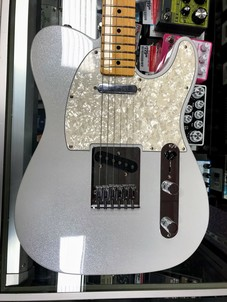
\includegraphics[width=0.4\linewidth]{guitar.jpg}
    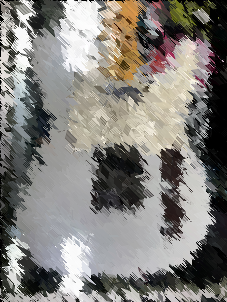
\includegraphics[width=0.4\linewidth]{big_guitar.png}
    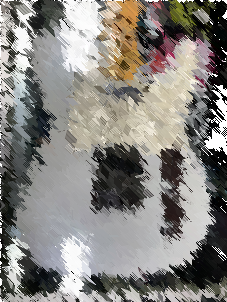
\includegraphics[width=0.4\linewidth]{guitar.png}
    \label{fig:guitarpics}
\end{figure}
\begin{figure}
    \centering
    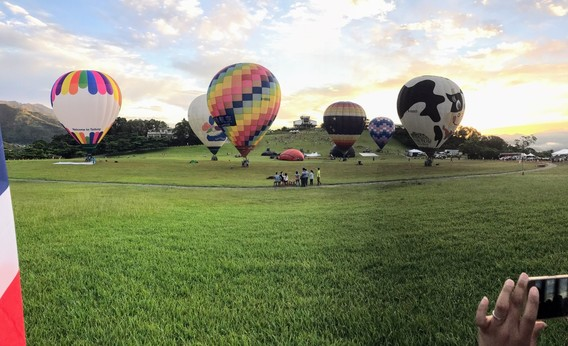
\includegraphics[width=0.8\linewidth]{hotairballoons.jpg}
    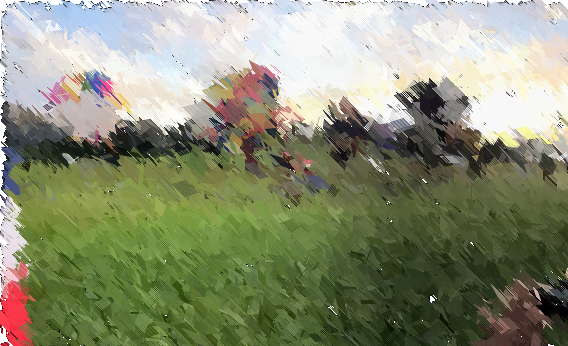
\includegraphics[width=0.8\linewidth]{hotair.png}
    \label{fig:hotairpics}
\end{figure}
\begin{figure}
    \centering
    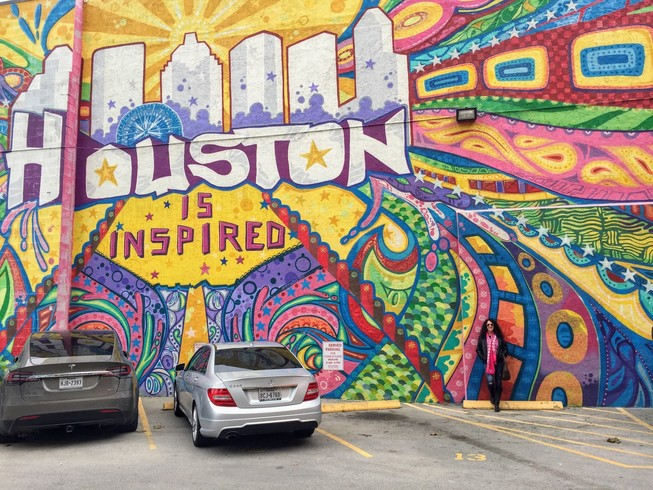
\includegraphics[width=0.6\linewidth]{houston.jpg}
    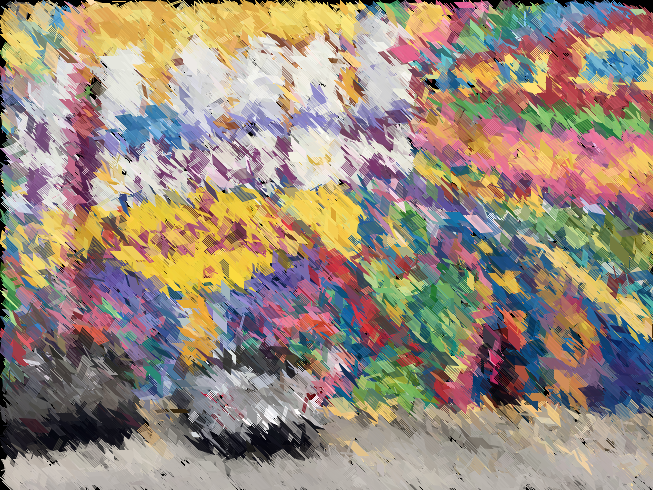
\includegraphics[width=0.6\linewidth]{houston_big.png}
    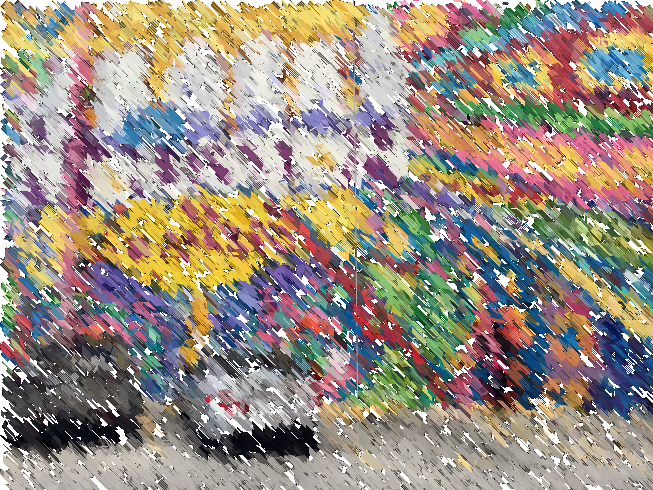
\includegraphics[width=0.6\linewidth]{houston.png}
    \label{fig:houstonpics}
\end{figure}



\end{document}
